\subsection{Análisis de rendimiento}
A continuación realizaremos un análisis de los tiempos insumidos por los métodos, el cual estará dividido en dos partes: primero, en forma preliminar para tener una orientación de que variables estudiar, un análisis superficial de la complejidad algorítmica de cada método; y luego, la contrastación empírica.

La PC sobre la que se tomaron los tiempos cuenta con un procesador Intel(R) Core(TM) i5-2500 @ 3.30GHz y 8GB de RAM.

\subsubsection{Complejidades de los métodos}
Utilizaremos la siguiente notación:
\begin{itemize}
	\item $cuadros\_originales$: la cantidad de cuadros que tiene el video original.
	\item $pixeles$: la cantidad de píxeles que tiene cada \emph{frame} del video.
	\item $cuadros$: la cantidad de cuadros que se desea agregar entre los existentes del video original.
\end{itemize}

En el caso de \emph{nearest neighbour} es bastante fácil darse cuenta que la complejidad es 

\begin{center}
	$O(cuadros\_originales \times pixeles \times cuadros)$
\end{center}

pues por cada píxel de cada cuadro copiamos $cuadros$ píxeles (lo que nos cuesta $O(1)$).

Para interpolación lineal pasa más o menos lo mismo, con la diferencia de que en lugar de copiar el píxel realiza unas pocas operaciones básicas que no dejan de ser $O(1)$, por lo que su complejidad es igual a la anterior.

Para analizar splines, vamos a considerar la partición en $n$ bloques de tamaño $b_1,..., b_n$ (o sea, ni siquiera suponemos que todos los bloques sean del mismo tamaño). Como por cada píxel se llama a la función \texttt{splines}, simplemente calculemos su complejidad y luego la multiplicamos por $pixeles$.

El costo de \texttt{splines} es la sumatoria de los costos de llamar a \texttt{splines\_bloque} por cada bloque. La complejidad de esta última función es 
\begin{center}
	$O(b\_i + b\_i \times cuadros) = O(b\_i \times cuadros)$
\end{center}

pues primero se resuelve el sistema con costo lineal \footnote{la complejidad exacta del algoritmo usado para resolver el sistema tridiagonal puede encontrarse en el capítulo 6 de \cite{burden}} sobre el tamaño del bloque, y luego por cada elemento del bloque se realizan $cuadros$ iteraciones de costo $O(1)$. Entonces nos queda que la complejidad de \texttt{splines} es

\begin{equation*}
\begin{split}
b_1 \times cuadros + b_2 \times cuadros + ... + b_n \times cuadros & = cuadros \times (b_1 + ... + b_n) \\
& = cuadros \times cuadros\_originales
\end{split}
\end{equation*}

Como esto había que multiplicarlo por $pixeles$, la complejidad total del método termina siendo igual a la de los dos métodos anteriores, aunque en este caso las constantes que se están ignorando son más significativas.

De esto deducimos entonces que las variables a analizar en la experimentación deben ser $cuadros$,  $cuadros\_originales$ y $pixeles$ (es decir, la resolución del video).

\subsubsection{Cantidad de cuadros a agregar}
Para esta sección consideramos variaciones con menos cuadros (para poder experimentar con mayor comodidad) de tres videos:
\begin{itemize}
	\item ff6: Versión de 22 cuadros, resolución 400x225
	\item darthvader: Versión de 15 cuadros, resolución 400x225
	\item penal: Versión de 18 cuadros, resolución 560x315
\end{itemize}

En base a los resultados de la sección anterior, es de esperar que para todos los métodos el tiempo de cómputo sea lineal sobre la cantidad de cuadros que se desean agregar. Sin embargo, está claro que las pendientes de cada método serán distintas pues las constantes lo son.  
Las hipótesis son realitavemente obvias: el método de vecino más cercano será el más veloz pues no realiza ningún cáculo sino que simplemente copia píxeles; lineal será el segundo más rápido pues a diferencia del anterior se agrega el cálculo de un polinomio de grado 1. Claramente los splines serán los que más tarden pues requieren evaluar un polinomio de grado 3 por cada cuadro a agregar. A su vez, es de esperar que independientemente del tamaño de bloque considerado para splines (4, 8 o 12), el tiempo de cómputo sea el mismo. Esto es consecuencia inmediata de que la complejidad del método, como vimos en la sección anterior, no depende de la partición escogida.


A continuación presentamos los resultados. Los mismos se obtuvieron de realizar 20 iteraciones para cada método y cantidad de cuadros a agregar.
\begin{figure}[H]
 \centering
	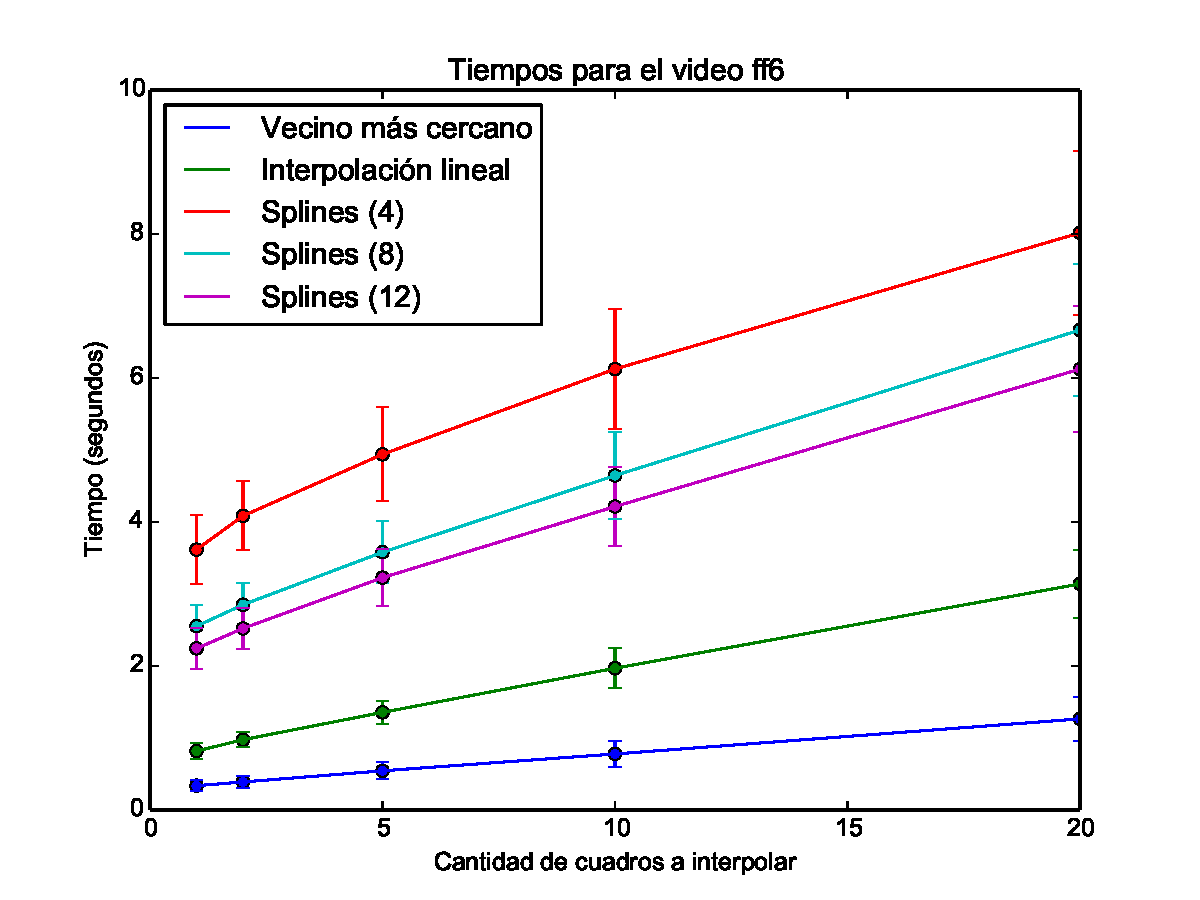
\includegraphics[width=0.7\textwidth]{imgs/resultados_tiempos/ff6_times.pdf}
	\caption{\footnotesize Tiempo que cuesta aplicar cada método sobre ff6 en función de la cantidad de cuadros que se desean agregar. Los puntos representan la media 0.20-podada de cada muestra. Las barras verticales indican la varianza.}
	\label{fig:ff6-times}
\end{figure}

\begin{figure}[H]
 \centering
	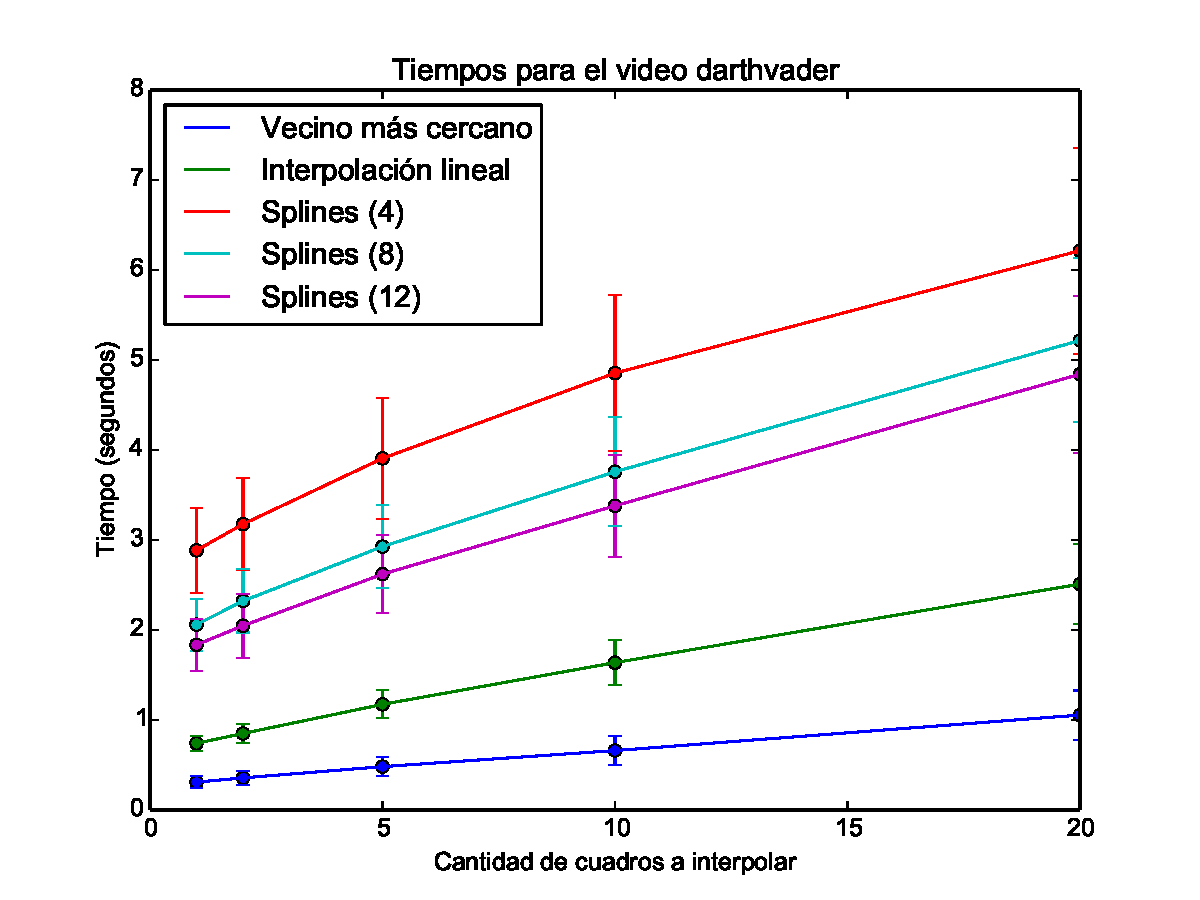
\includegraphics[width=0.7\textwidth]{imgs/resultados_tiempos/darthvader_times.pdf}
    \caption{\footnotesize Tiempo que cuesta aplicar cada método sobre darthvader en función de la cantidad de cuadros que se desean agregar. Los puntos representan la media 0.20-podada de cada muestra. Las barras verticales indican la varianza.}
    \label{fig:darthvader-times}
\end{figure}

\begin{figure}[H]
 \centering
	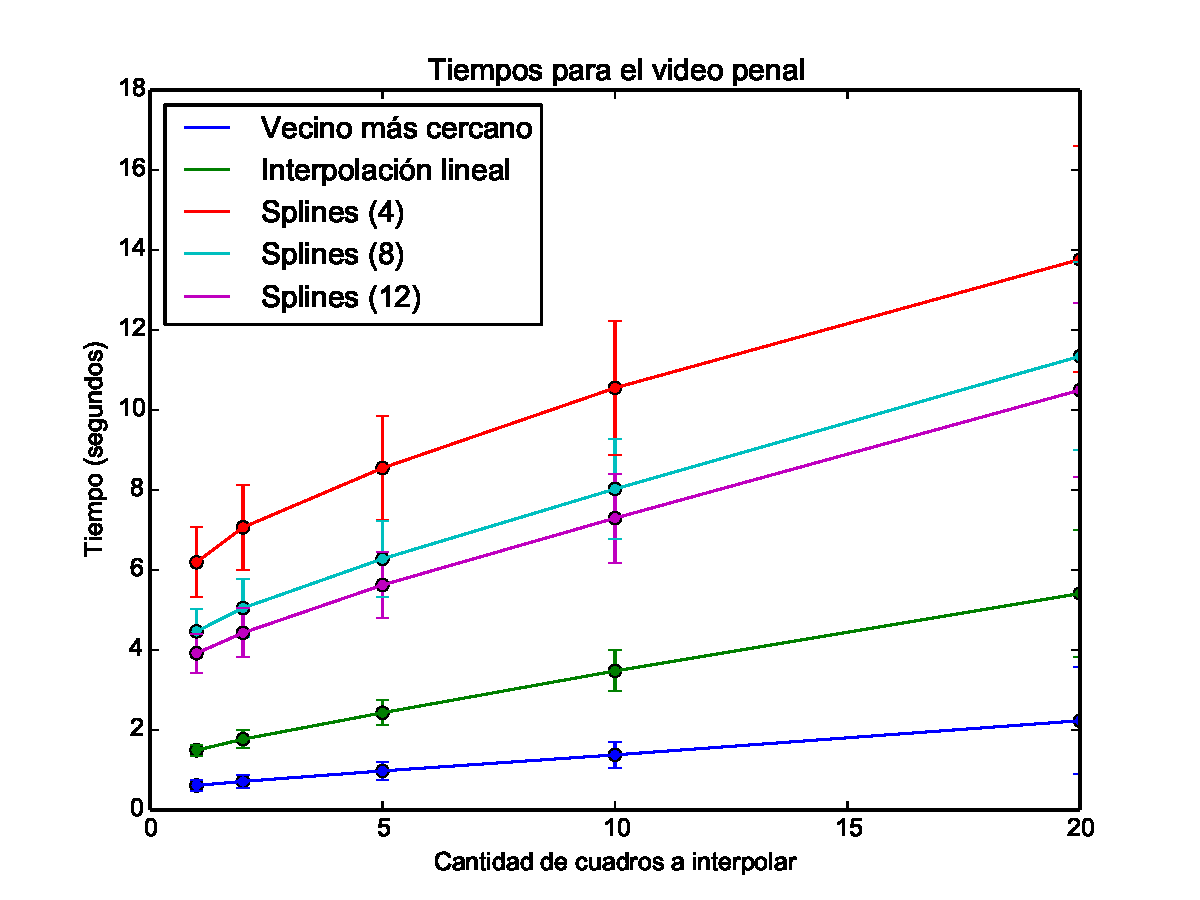
\includegraphics[width=0.7\textwidth]{imgs/resultados_tiempos/penal_times.pdf}
    \caption{\footnotesize Tiempo que cuesta aplicar cada método sobre penal en función de la cantidad de cuadros que se desean agregar. Los puntos representan la media 0.20-podada de cada muestra. Las barras verticales indican la varianza.}
    \label{fig:penal-times}
\end{figure}

Al ver los gráficos vemos que se sostienen las hipótesis respecto de los métodos de vecino más cercano e interpolación lineal, pero curiosamente las tres variantes de splines muestran tiempos distintos. No solo eso, sino que consistentemente en todos los casos a mayor tamaño de bloque, menos tarda en computar el método.

Si observamos con un poco más de detenimiento las figuras \ref{fig:darthvader-times} y \ref{fig:penal-times} vemos que las varianzas de los splines son altas y en muchos casos se superponen las tres, pero la figura \ref{fig:ff6-times} que muestra una varianza un poco más acotada parece señalar que la tendencia marcada en el párrafo anterior efectivamente existe. Parece razonable atribuirle gran parte de esto al hecho de que, al considerar particiones de bloques más pequeños, se llama más veces a la función  \texttt{splines\_bloque} y se entra más al ciclo \texttt{while} de \texttt{splines}, lo que provoca que las constantes que despreciamos al calcular la complejidad incidan más en la brecha de tiempos observada. Más específicamente, son las constantes que sumaban las que provocan la diferencia, pues al ver el gráfico vemos que lo que ocurre es un corrimiento sobre el eje de ordenadas pero no un cambio de curvatura.


\subsubsection{Tamaño de bloque}
Las hipótesis son escencialmente análogas al caso anterior. Ahora con la corrección de que seguramente veamos un fenómeno similar al visto antes con respecto a los tres métodos de splines.

\begin{figure}[H]
 \centering
	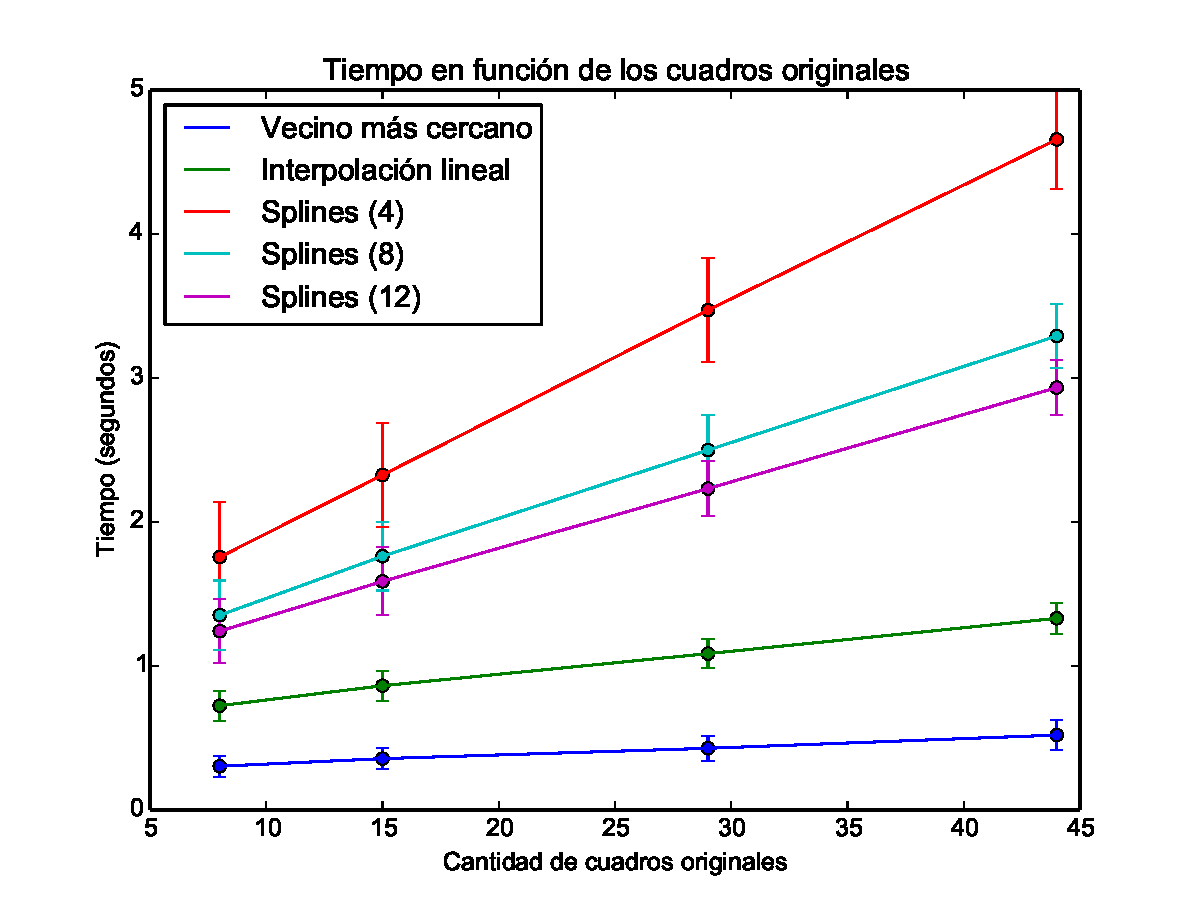
\includegraphics[width=0.7\textwidth]{imgs/resultados_tiempos/ff6_times_cuadros.pdf}
	\caption{\footnotesize Tiempo que se requiere al aplicar cada método sobre un video para interpolar 2 cuadros en función de la cantidad de cuadros que poseía originalmente. Los puntos representan la media 0.20-podada de cada muestra. Las barras verticales indican la varianza.}
	\label{fig:ff6-times-cuadros}
\end{figure}

La figura \ref{fig:ff6-times-cuadros} efectivamente corrobora lo esperado. 

Algo interesante que puede observarse en este gráfico es que, a diferencia de lo que pasaba al aumentar los cuadros a agregar, las pendientes con las que crecen las curvas de las tres variantes de splines no son iguales. Es decir, en las figuras de la \ref{fig:ff6-times} a la \ref{fig:penal-times} puede apreciarse que la curvatura de los puntos es prácticamente igual aunque haya un desplazamiento sobre el eje de ordenadas. Sin embargo, aquí vemos que los puntos correspondientes a la versión que usa bloques de tamaño 4 están cada vez más espaciados de los otros. Incluso entre los correspondientes a \emph{splines (8)} y \emph{splines (12)} puede notarse esta diferencia de pendiente aunque en menor medida.

Esto resulta razonable a la luz de los hechos vistos en el punto anterior: si habíamos dicho que el tiempo del método aumentaba cuantas más veces se caía en el \texttt{while} de la función \texttt{splines} es lógico que al aumentar la variable de la cual este hecho depende directamente esta situación se potencie. Visto con un ejemplo: si dado un video le aumentáramos en 8 la cantidad de sus cuadros originales, para \emph{splines (8)} y \emph{splines (12)} esto implicaría a lo sumo caer una vez más en el \texttt{while}, mientras que para \emph{splines (4)} resulta en hacerlo dos veces más. Si lo hiciéramos en 24 cuadros, serían 2 veces para \emph{splines (12)}, 3 para \emph{splines (8)} y 6 para \emph{splines (4)}. Es decir que el aumento siempre es desigual, y eso justifica la diferencia en las pendientes.

\subsubsection{Resolución}
Finalmente, analicemos la influencia de la resolución. Es de suponer que el comportamiento sea similar al del caso anterior, o sea, que las pendientes de crecimiento sean distintas para todos los métodos, pues la cantidad de píxeles que conforman un \emph{frame} es lo que determina la cantidad de veces que se llame a las funciones que implementan los métodos de interpolación, por lo cual es razonable que todas las constantes propias de cada método se vean potenciadas.

En efecto, la figura \ref{fig:times-resolucion} verifica estas suposiciones.  

\begin{figure}[H]
 \centering
	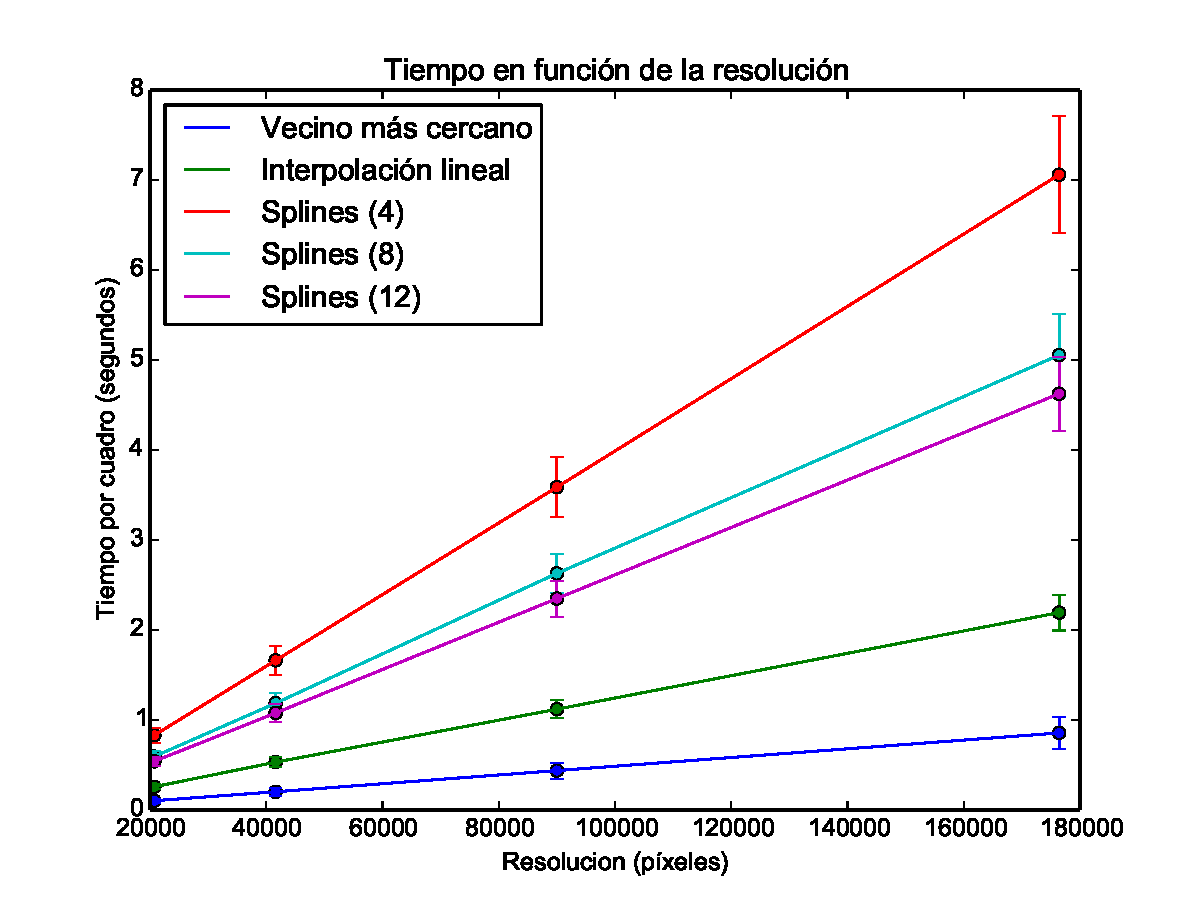
\includegraphics[width=0.7\textwidth]{imgs/resultados_tiempos/resolucion.pdf}
	\caption{\footnotesize Tiempo que se requiere al aplicar cada método sobre un video para interpolar 2 cuadros en función de la resolución del mismo. Los puntos representan la media 0.20-podada de cada muestra. Las barras verticales indican la varianza.}
	\label{fig:times-resolucion}
\end{figure}